\documentclass{amsart}

%\documentclass[a4paper,11pt]{amsart}

\usepackage{graphics}
\usepackage{amsthm}
\usepackage{thmtools}
%\usepackage{wasysym}
%\usepackage{arxiv}
%\usepackage{enseign}

\usepackage{iftex}                      % check which engine is compiling this file
\iftutex                                % xelatex or lualatex specific first
 \usepackage{fontspec}                  % font selection in xelatex/lualatex
 \defaultfontfeatures {Ligatures=TeX}
 \usepackage{unicode-math}              % amssymb+amsmath equiv., to show $θ$ as θ
 \unimathsetup{math-style=TeX}
 \setmathfont{Stix Two Math}
 \ifLuaTeX
  % \usepackage{luatex85}               % compatibility of luatex with xy
   \usepackage{lualatex-math}
 \fi
\else                                   % 8bit (e.g. pdflatex) specific
 \usepackage[T1]{fontenc}               % use 8-bit T1 fonts
 % \usepackage[utf8]{inputenc}           % allow utf-8 input, for texlive-2016 and older
 \usepackage{amsmath,amssymb}
\fi
\usepackage{alphabeta}                  % type αβγ directly, in LuaLaTeX use {unicode-math} (above)


\usepackage{amsbsy,amscd,amsfonts}
\usepackage[pagebackref=true]{hyperref}
\usepackage[nameinlink,capitalize,noabbrev]{cleveref}
%\usepackage{hyperref}
%\usepackage{url}            % simple URL typesetting
%\usepackage{booktabs}       % professional-quality tables
%\usepackage{nicefrac}       % compact symbols for 1/2, etc.
%\usepackage{microtype}      % microtypography

\usepackage{graphicx,float,latexsym,color}
%\usepackage{refcheck}
%\usepackage{mathspec}
\usepackage[font={scriptsize,it}]{caption}
\usepackage{subcaption}
%\let\proof\relax
%\let\endproof\relax

\usepackage{makecell}

% usar \defcommand em vez de \newcommand ou \renewcommand
% funciona como \def em tex - vai definir, se ainda não definida,
% se já definida, vai redefinir
\makeatletter\def\defcommand{\@ifstar\defcommand@S\defcommand@N} \def\defcommand@S#1{\let#1\outer\renewcommand*#1} \def\defcommand@N#1{\let#1\outer\renewcommand#1} \makeatother

\renewcommand{\arraystretch}{1.2}

\usepackage[dvipsnames]{xcolor}

\newtheorem{theorem}{Theorem}
\newtheorem*{theorem*}{Theorem}
\newtheorem{lemma}{Lemma}
\newtheorem{proposition}{Proposition}
\newtheorem{corollary}{Corollary}

\theoremstyle{remark}
\newtheorem{remark}{Remark}
\newtheorem{observation}{Observation}
\newtheorem{example}{Example}

\theoremstyle{definition}
\newtheorem{definition}{Definition}
\newtheorem{question}{Question}
\newtheorem{conjecture}{Conjecture}

\hypersetup{
    %bookmarks=true,         % show bookmarks bar?
    %unicode=true,          % non-Latin characters in Acrobat’s bookmarks
    pdftoolbar=true,        % show Acrobat’s toolbar?
    pdfmenubar=true,        % show Acrobat’s menu?
    pdffitwindow=false,     % window fit to page when opened
    pdfstartview={FitH},    % fits the width of 
    colorlinks=true,        % false: boxed links; true: colored links
    linkcolor=OliveGreen,   % color of internal links (change box color with linkbordercolor)
    citecolor=blue,         % color of links to bibliography
    filecolor=black,        % color of file links
    urlcolor=TealBlue       % color of external links
}

\usepackage{lineno}
\def\linenumberfont{\normalfont\small\sffamily}
%a4: 210 x 297
%\textwidth=125mm
%\textheight=195mm
\arraycolsep=2pt
\captionsetup{width=120mm}

 
\usepackage{comment}
\usepackage{microtype}
\usepackage{footnote}
%\usepackage{tablefootnote}
%\usepackage{longtable}

\usepackage[mark]{gitinfo2}

% my local settings for night reading
% \usepackage{sergey}

%% math blackboard
% \newcommand{\D}{\mathbb{D}}           % unused

%% math bold face
\defcommand{\k}{\mathbf{k}}             % base field
\defcommand{\A}{\mathbf{A}}             % [A]ffine plane/space
% \defcommand{\F}{\mathbf{F}}             % [F]inite [f]ield       (unused)
\defcommand{\C}{\mathbf{C}}             % [C]omplex numbers
% \defcommand{\P}{\mathbf{P}}		% projective plane/space   (unused)
\newcommand{\Q}{\mathbf{Q}}             % Rational numbers
\newcommand{\R}{\mathbf{R}}             % [R]eal numbers
\newcommand{\Z}{\mathbf{Z}}             % Integer [Z]ahlen

%% math calligraphic
\defcommand{\AA}{\mathcal{A}}           % For \AA_s in evolute
\newcommand{\EE}{\mathcal{E}}		% [E]llipse
\newcommand{\FF}{\mathcal{F}(a,b)}           % [F]amily
\newcommand{\PP}{\mathcal{P}}           % [P]olytope
\newcommand{\QQ}{\mathcal{Q}}           % Regular polytope (maybe better R?)
% \newcommand{\TT}{\mathcal{T}}		% unused
% \newcommand{\XX}{\mathcal{X}}         % unused

\newcommand{\ol}{\overline}

\newcommand{\torp}[2]{\texorpdfstring{#1}{#2}}
% \newcommand{\ab}{_{\alpha,\beta}}     % unused

\DeclareMathOperator{\ord}{ord}
\DeclareMathOperator{\Ker}{Ker}
\DeclareMathOperator{\tr}{Tr}
\DeclareMathOperator{\GL}{GL}           % [G]eneral [L]inear group
\DeclareMathOperator{\SO}{SO}           % [S]pecial [O]rthogonal group
\DeclareMathOperator{\SL}{SL}           % [S]pecial [L]inear group
% \DeclareMathOperator{\O}{O}             %           [O]rthogonal group
\DeclareMathOperator{\Un}{U}             %           [U]nitary group

\newcommand{\Mod}[1]{\ (\mathrm{mod}\ #1)}

\newcommand{\complain}[1]{\textcolor{red}{#1}}


\title[Invariants of Poncelet N-Periodics in the Homothetic Pair]{Invariants of Poncelet N-Periodics\\in the Homothetic Pair}
\author{Sergey Galkin}
\author{Ronaldo Garcia}
\author{Dan Reznik}

\date{February, 2021}

\begin{document}

\maketitle

\begin{abstract}
We describe and prove two new invariants manifested by the ``homothetic'' family, i.e., a family of Poncelet N-gons interscribed between two concentric, axis-aligned, homothetic ellipses. In contradistinction with the confocal family (elliptic billiard) which conserves perimeter, Joachimsthal's constant, and the sum of internal angle cosines, the homothetic family conserves area, sum of squared sidelengths, and the sum of internal angle cotangents.
\end{abstract}


\section{Introduction}
\label{sec:intro}
We describe new invariants manifested by the 1d family of Poncelet N-periodics interscribed in the so-called ``homothetic pair'', i.e., a pair of concentric, axis-aligned ellipses with identical aspect ratio. In \cref{fig:confocal_homot} the family is illustrated next to the ``confocal'' family, also known as the {\em elliptic billiard}.

\begin{figure}
    \centering
    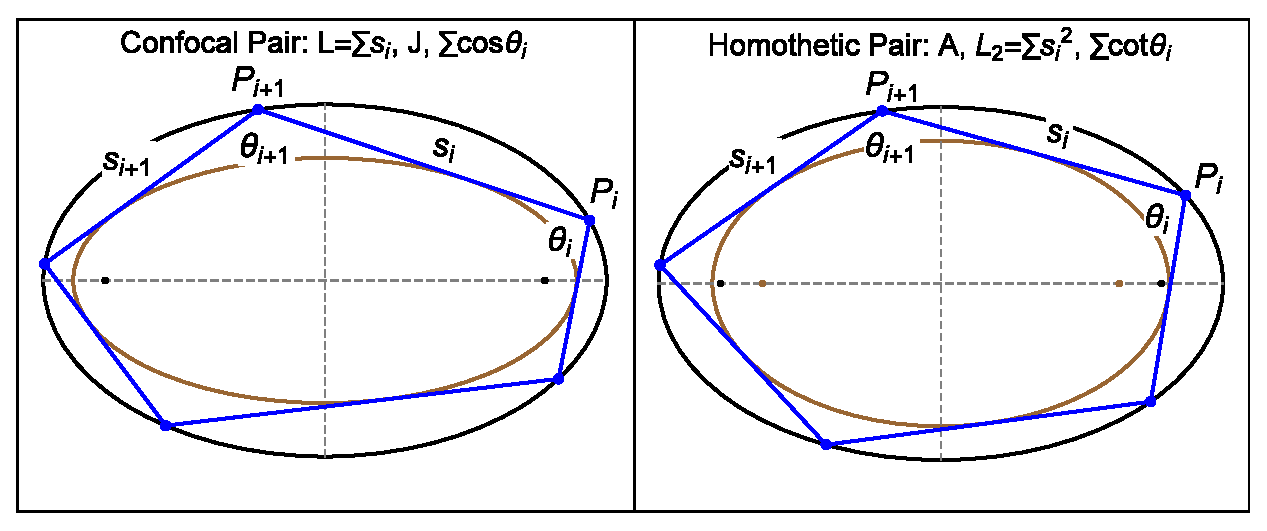
\includegraphics[width=\textwidth]{pics/0010_confocal_homot.eps}
    \caption{\textbf{Left:} A Poncelet 5-periodic in the confocal pair (elliptic billiard). It classically conserves perimeter $L=\sum{s_i}$ and Joachimsthal's constant $J$ \cite{sergei91}. It also conserves $\sum\cos\theta_i$ \cite{akopyan2020-invariants,bialy2020-invariants,reznik2020-intelligencer}. \textbf{Right:} The homothetic family, interscribed between two concentric, axis-aligned, non-confocal, homothetic ellipses. It trivially conserves area $A$. We show it also conserves (i) sum of squared sidelengths $s_i^2$ and (ii) sum of {\em cotangents} of the $\theta_i$.}
    \label{fig:confocal_homot}
\end{figure}

 Two classic elliptic billiard invariants are perimeter $L$ and Joachimsthal's constant $J$  \cite{sergei91}. Recall the latter is tantamount to tangency of sidelines to a confocal caustic. Recently, we've shown this family also conserves the sum of cosines \cite{akopyan2020-invariants,bialy2020-invariants}, as well as product of ``outer'' cosines and certain area ratios \cite{caliz2020-area-product,reznik2020-intelligencer}. For a complete list see \cite{reznik2021-fifty}.

Returning the homothetic family, notice it trivially conserves area $A$ since it is  the affine image of Poncelet polygons between two concentric circles.

\subsection*{Main Results} Using properties of trigonometric polynomials (see \cref{sec:trig-polys}), we show that the homothetic family conserves:

\begin{enumerate}
    \item \cref{lem:norm2}: sum of squared distances from the vertices to any point; see \cref{fig:homot_norm}.
    \item \cref{prop:sqr_si}: the sum of {\em squared} sidelengths.
    \item \cref{th:cot}: the sum of internal angle cotangents.
    \item \cref{prop:dist-focus}: the sum of distances from the vertices to a focus of the external ellipse.
    \item \cref{cor:kappa}: the sum of curvatures $\kappa_i^{-2/3}$ at each vertex.
\end{enumerate}

In the $N=3$ case, a harmonious corollary of the first two results is that the family conserves the Brocard angle $\omega$; see \cref{fig:brocard-n3}. In fact, the idea for the third result is the fact that in a triangle, $\cot\omega=\cot\theta_1+\cot\theta_2+\cot\theta_3$ \cite[Brocard Angle]{mw}. Though for $N>3$ the Brocard angle $\omega$ is no longer defined, magically, the sum of angle cotangents remains invariant.

\begin{figure}
    \centering
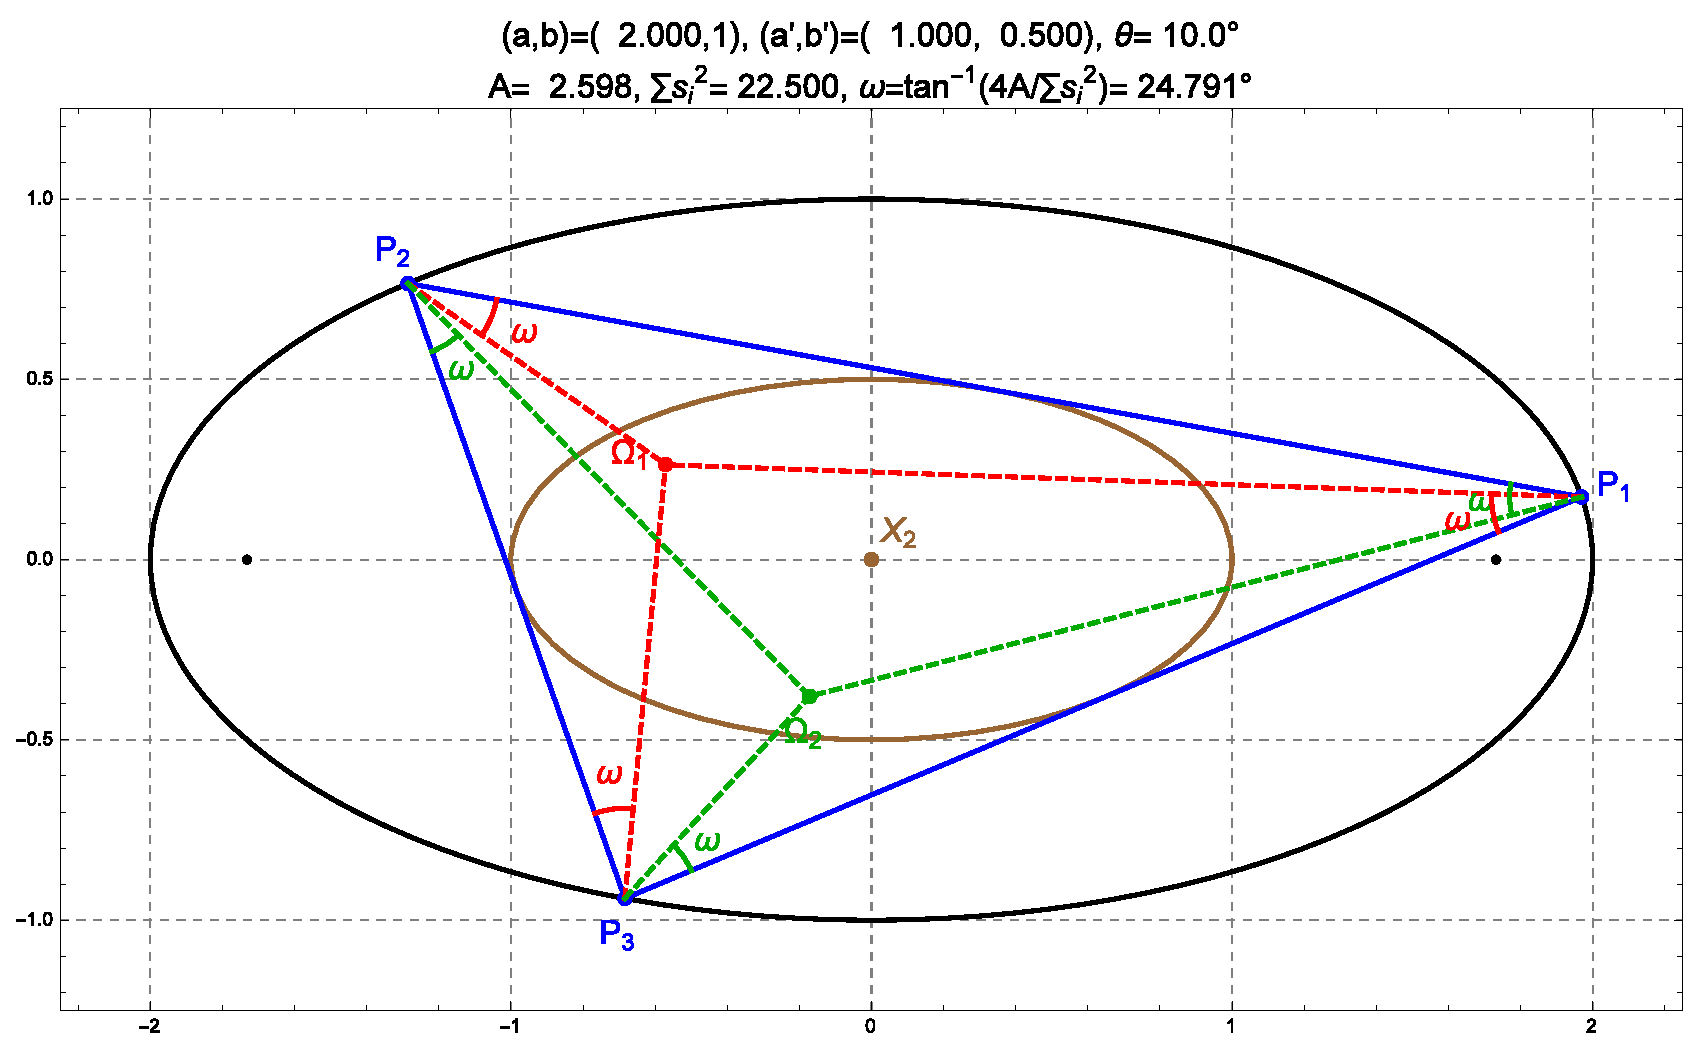
\includegraphics[width=\textwidth]{pics/0040_brocard_n3.eps}
\caption{The family of 3-periodics in the homothetic pair conserve area, sum of squared sidelengths and the Brocard angle $\omega$ which is the particular angle of rotation of sidelengths such that they concur at the two Brocard points $\Omega_1$ and $\Omega_2$. $X_2$ is barycenter which remains stationary over the family at the common center. \href{https://youtu.be/2fvGd8wioZY}{Video 1} and \href{https://youtu.be/13i3JGY-fK4}{Video 2}.}
    \label{fig:brocard-n3}
\end{figure}

Below we only describe Poncelet families of simple N-gons. However all claims hold for self-intersected ones as well.



\section{Trigonometric Polynomials}
\label{sec:trig-polys}
Recall that a rotation of a unit circle can be parametrized either (i)
by its angle $\varphi$,
or (ii) by a pair of Cartesian coordinates $(x,y)$ such that $x^2+y^2=1$,
or (iii) by a unit complex number $z$, noting that 
$z = x + y \cdot i = \exp(i \varphi) = \cos(\varphi) + \sin(\varphi) \cdot i$
($i^2=-1$),
thus $\cos(\varphi) = (z+z^{-1})/2$, $\sin(\varphi) = (z-z^{-1})/(2i)$.
Fixing a reference point $P_0$ one can identify a rotation $\rho$
with a point $\rho(P_0)$.
Thus the composition of rotations as well as the action of a rotation on a point
are described by multiplication of complex numbers.
In particular the rotation by a fixed angle is linear transformatin
in either complex coordinate $z$ or in the real coordinates $x,y$.
Also, the sequence of points $\dots,P_{k-1},P_k,P_{k+1},\dots$
is obtained by consecutive fixed rotations $ρ$
if and only if the corresponding sequence of complex numbers
is a geometric progression:
\[ P_i^2 = P_{i-1} \cdot P_{i+1} \]
For any bivariate polynomial of degree less than $d$,
the result of the substitution $(x,y) \mapsto (\cos(\varphi),\sin(\varphi))$
can be uniquely written as a linear combination of Laurent monomials $z^k$ with $|k|<d$. We will call
such elements trigonometric (or Laurent) polynomials of degree less than $d$.
An example of a function which is not a trigonometric polynomial
is given by the cotangent:


\[\cot(\varphi) := \frac{\cos(\varphi)}{\sin(\varphi)} 
= i \frac{z^2+1}{z^2-1} = i \left(1+\frac{1}{1-z}-\frac{1}{1+z}\right)\]

Let $ζ$ (resp. $z$) be a complex number associated with a rotation (resp. an initial point),
and $f$ be a function on a circle.

The $N$-step average from starting point $z_0$ for a function $f$ is defined as:

\[ \int_{ζ,N,z_0} f := \frac{1}{N} \sum_{k=0}^{N-1} f(ζ^k \cdot z_0), \]
if $ζ^N = 1$ we will simply write $\int_{N,z}$.

Note that if $f(w) = w^M$ then $f(ζ^k \cdot z_0) = f(ζ^k) \cdot f(z_0)$,
so $\int_{ζ,N,z_0} f = f(z_0) \times \int_{ζ,N,1} f$,
moreover the second factor 
\[ 
\int_{ζ,N,1} z^M 
= \frac{1}{N} \sum_{k=0}^{N-1} ζ^{kM} 
= \frac{1}{N} \frac{1-ζ^{NM}}{1-ζ^M} 
\]
equals $1$ if $ζ^M=1$, 
and otherwise equals to $\frac{1}{N} \frac{1-ζ^{NM}}{1-ζ^M}$. In particular it is zero if $ζ^N=1$.



This implies that if $f$ is a trigonometric polynomial of degree $d$,
then for any $N>d$ and any starting point $z_0$
all $N$-periodic time averages of $f$ yield the same value.
This value equals the zeroth Fourier coefficient (in front of $z^0$),
which is the space average.

In what follows we apply this argument to our three main results. In the first two, the application is straightforward. In the third case (invariant sum of cotangents), we proceed through the following steps to obtain a trigonometric polynomial:

\begin{enumerate}
    \item The cotangent is equal to the scalar product divided by area.
\item Since area is constant (multiplied by the affine Jacobian), the cotangent is proportional to the scalar product.

\item Scalar product (before or after dilation) is a quadratic polynomial in coordinates
of three points (the center one is a vertex).

\item The coordinates of these three points $P_{i-1},P_i,P_{i+1}$
are linear in the coordinates of the center point $P_i$, % already proved above
%; see \cref{eq:scaled-dynamics}.
\item Therefore, the cotangent is a quadratic function and for $N>2$ its time average is independent
of the starting point and equals to space average.
\end{enumerate}





\section{Invariant Sum of Squared Sidelengths}
Let a pair of homothetic, concentric, axis-aligned ellipses $\E$ and $\E_c$ have center at the origin. Let $a,b$ denote the semi-axes of $\E$. The semi-axes $a_c,b_c$ of $\E_c$ such that the pair admits a family of Poncelet N-periodics are be given by:

\[ a_c = a\cos\frac{\pi}{N},\;\;\;b_c = b\cos\frac{\pi}{N} \]

Since the family is an affine image of regular polygons interscribed in a concentric pair of circles, its area is invariant and given by:
\[A_N= N \sin \left( {\frac {2\pi}{N}} \right) \frac{ab}{2}\]

Referring to \cref{fig:homot_norm} (left):

\begin{lemma}
\label{lem:norm2}
Over Poncelet N-Periodics $\{p_1,\ldots p_n\}$ in the homothetic pair, the sum of squared norms $|p_k|^2$  is invariant and given by:

\[   \sum_{k=1}^N |p_k|^2=\frac{ N(a^2 + b^2)}{2}
	\]
\end{lemma}

\begin{figure}
    \centering
    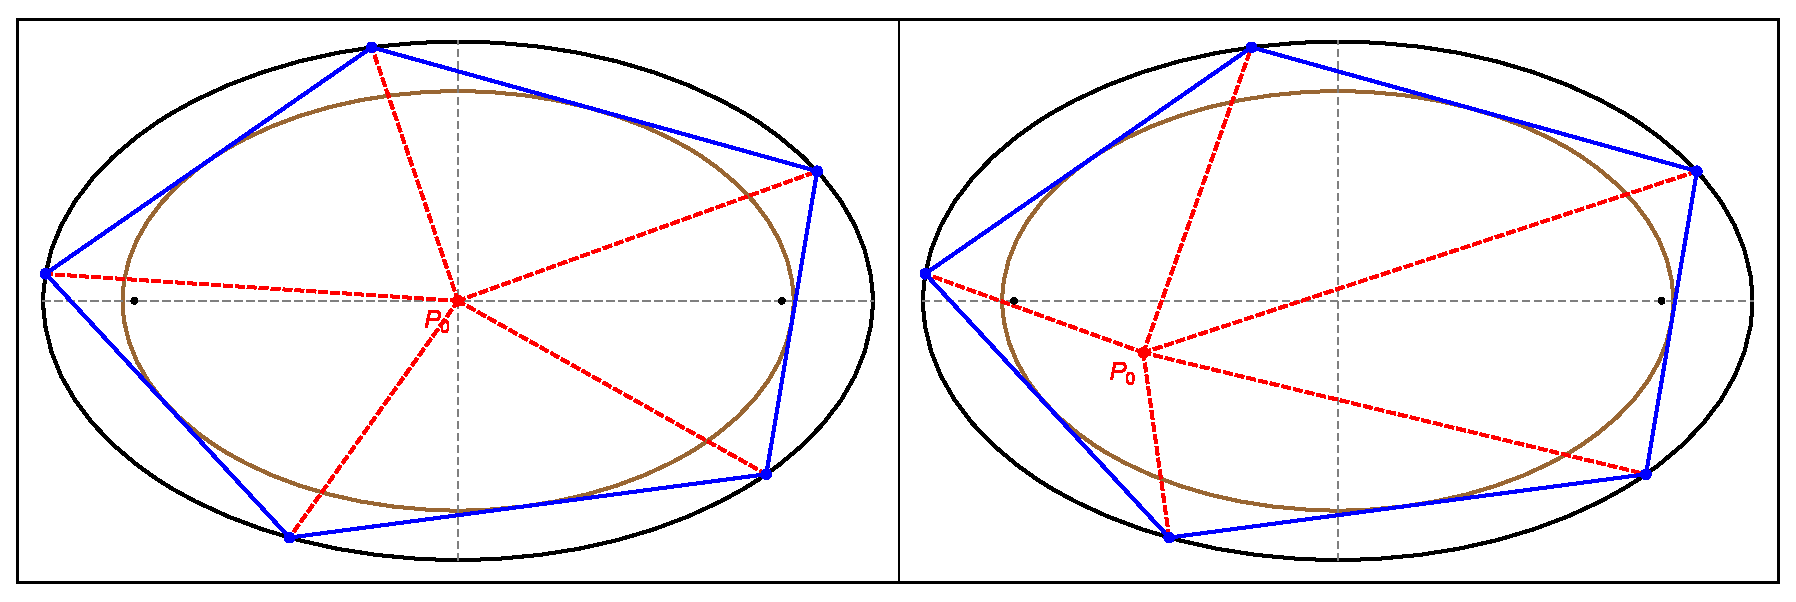
\includegraphics[width=\textwidth]{pics/0020_homot_norm.eps}
    \caption{\textbf{Left:} \cref{lem:norm2} states that the sum of squared norms of the vertices with respect to the center is invariant. \textbf{Right:} \cref{cor:p0} states that in fact the squared norms of vertices with respect to any point $P_0$ is invariant. \href{https://youtu.be/2PdsC3CcqaE}{Video}}.
    \label{fig:homot_norm}
\end{figure}

\noindent The proof below was kindly contributed by Sergei Tabachnikov
\cite{sergei2020-private-sidelengths}.

\begin{proof}
For the sake of the argument, we first consider the $N=3$ case. Define $v(\alpha)=(\cos \alpha, \sin \alpha)$ and a matrix $A$ which takes concentric circles to homothetic ellipses. Then $|Av(\alpha)|^2$ is a trigonometric polynomial of degree 2, and we average it over $\mathbb{Z}_3$ by adding $2\pi/3$ and $4\pi/3$ to $\alpha$. The result is independent of $\alpha$, as needed. Extending it to all $N$, note that a trigonometric polynomial of degree 2 averages to a constant over the action of $\mathbb{Z}_N$. The explicit expression was obtained via the the vertex parametrization below and CAS simplification.

%Let $P_1(t)=(x_1,y_1)=(a\cos{t},b\sin{t})$. Then $P_{k+1}=(x_{k+1},y_{k+1})$, $k=0...(N-1)$ are given by:

%\[ P_{k+1}=\left[a\cos \left( {\frac {2\,\pi\,k+tN}{N}} \right) ,b\sin \left( {\frac {2\,\pi\,k+tN}{N}} \right) \right]\]
\end{proof}

\begin{proposition}
\label{prop:sqr_si}
Over Poncelet N-Periodics in the homothetic pair, the sum of squared sidelengths $L_{2,N}$ is invariant. It is given by:

\[ L_{2,N}= \sum_{k=1}^N L_k^2=N \left[ 1-\cos \left(  {\frac {2\pi}{N}} \right)  \right]  \left(
{a}^{2}+{b}^{2} \right) 
	\]
\end{proposition}

\begin{proof}
The sidelengths are expressed by trigonometric polynomials of degree 2. So the proof is analogous to that of   \Cref{lem:norm2}.
\end{proof}
\noindent Referring to \cref{fig:brocard-n3}, recall the Brocard angle $\omega$ of a triangle is given by $\cot\omega=L_{2,3}/(4A_3)$ \cite[Brocard Angle]{mw}. Then:

\begin{corollary}
The family of 3-periodics in the homothetic pair conserves Brocard angle $\omega$.    
\end{corollary}

Note: a well-known identity is that $\cot\omega=\cot\theta_1+\cot\theta_2+\cot\theta_3$. \cref{th:cot} is statement that this sum generalizes for $N>3$. 

%\begin{corollary}
%	\[ 4\left(1-\cos\left(\frac{2\pi}{n}\right) \right)A_n Cot_n+ n\cos\left(\frac{2\pi}{n}\right) L_n=0\]
%\end{corollary}

Referring to \cref{fig:homot_norm}, the sum of squared distances from vertices to a fixed point $p_0$ is also invariant, owing to the same trigonometric polynomial argument:

\begin{corollary}
\[   \sum_{k=1}^N |p_k-p_0|^2=\frac{ N(a^2 + b^2)}{2} + N |p_0|^2
\]
\label{cor:p0}
\end{corollary}






\section{Invariant Sum of Cotangents}
\label{sec:cotangent}
In this section we prove that the sum of cotangents over the homothetic N-periodic family is invariant.
We use the following parametrization for the vertices.
Rotation by angle $\alpha$ is given by
\[ z\to z' = e^{i \alpha} \cdot z \]
Since $e^{i \alpha} = \cos \alpha + i \sin \alpha$
for $z = x + i y$ and $z'=x'+iy'$ we have
\[
   x'+iy' = z' 
 = e^{i \alpha} \cdot z
 = (\cos \alpha + i \sin \alpha) (x + i y) 
 = (x \cos \alpha - y \sin \alpha) + i (x \sin \alpha + y \cos \alpha)
\] 
or
\begin{align*} x' &= (x \cos \alpha - y \sin \alpha)    &     y' &= (x \sin \alpha + y \cos \alpha) \end{align*}
Also if $z = e^{i \beta}$ then $z' = e^{i (\beta+\alpha)}$ and respectively $x'=\cos(\beta+\alpha), y'=\sin(\beta+\alpha)$.
So we can explicitly write down coordinates for the next and the previous points using $\cos(-\alpha)=\cos(\alpha)$ and $\sin(-\alpha)=-\sin(\alpha)$.
If $T (x_i,y_i) = (x_{i+1},y_{i+1})$, then
\begin{align*} 
x_{i+1} &= (x_i \cos \alpha - y_i \sin \alpha)    &     y_{i+1} &= (x_i \sin \alpha + y_i \cos \alpha)  \\
x_{i-1} &= (x_i \cos \alpha + y_i \sin \alpha)    &     y_{i-1} &= (-x_i \sin \alpha + y_i \cos \alpha)  
\end{align*}

And if $X_i = a x_i$ then

\begin{align} 
X_{i+1} &= a(x_i \cos \alpha - y_i \sin \alpha) & y_{i+1} &= b( x_i \sin \alpha + y_i \cos \alpha) \nonumber \\
X_i &= a x_i & y_i &= b y_i \label{eq:scaled-dynamics} \\
X_{i-1} &= a(x_i \cos \alpha + y_i \sin \alpha)   &    y_{i-1} &= b(-x_i \sin \alpha + y_i \cos \alpha) \nonumber
\end{align}



\begin{theorem}
Over Poncelet N-Periodics in the homothetic pair, the sum of cotangents of the internal angles $\theta_k$ is invariant. It is given by:
\[ \sum_{k=1}^N \cot\theta_k	=-  N \cot
		\left( {\frac {2\pi}{N}} \right)  \frac {\left( {a}^{2}+{b}^{2} \right) }{2ab}
\]	
\label{th:cot}
\end{theorem}

\begin{proof}
The cotangent of an angle $\theta=\angle{ABC}$ is rational on the vertex coordinates. Explicitly, if $B=O:=(0,0)$ and $C=H:=(*,0)$, $A=(x,y)$ then
\[ \cot\theta = \frac{x}{y} \]
If $C=(x_1,y_1)$ and $A=(x_3,y_3)$ consider the associated complex numbers $x_1 + i y_1$ and $x_3 + i y_3$, respectively. Their ratio $d$ is given by:
\[ d 
 = \frac{x_1 + i y_1}{x_3 + i y_3} 
 = \frac{(x_1 + i y_1)(x_3 - i y_3)}{(x_3 + i y_3)(x_3 - i y_3)} 
 = \frac{(x_1 x_3 + y_1 y_3) + i (y_1 x_3 - y_3 x_1)}{x_3^2 + y_3^2}
\]
Angle $AOC$ is homothetic to angle $HOD$, hence:

\begin{equation} \label{cotangent}
\cot\theta = \frac{x_1 x_3 + y_1 y_3}{y_1 x_3 - y_3 x_1} 
\end{equation}

The formula for the cotangent of an abstract triple is obtained by a shift, but it will be easier to do the shift directly.

\begin{equation*} 
\cot((x_1,y_1),(x_2,y_2),(x_3,y_3)) = 
\frac{(x_1-x_2) (x_3-x_2) + (y_1-y_2) (y_3-y_2)}{(y_1-y_2) (x_3-x_2) - (y_3-y_2) (x_1-x_2)}
\end{equation*}

Without loss of generality we will set $b=1$. Rewrite \cref{eq:scaled-dynamics} as: 

\begin{align*}
X_+ - X &= a (x (\cos \alpha - 1) - y \sin \alpha)& y_+ - y &= ( x \sin \alpha + y (\cos \alpha - 1))  \\
X_- - X &= a (x (\cos \alpha - 1) + y \sin \alpha) & y_- - y &= (-x \sin \alpha + y (\cos \alpha - 1))  
\end{align*}

\noindent or in trigonometric form:

\begin{align*}
X_+ - X &= a (\cos(\beta+\alpha)-\cos(\beta))    &     y_+ - y &= \sin(\beta+\alpha)-\sin(\beta)  \\
X_- - X &= a (\cos(\beta-\alpha)-\cos(\beta))    &     y_- - y &= \sin(\beta-\alpha)-\sin(\beta)  
\end{align*}

\noindent substitute the above into 
\cref{cotangent} and get:

\begin{equation*} \label{cot-a}
\cot(x,y,a) = \frac{a x_- x_+ + a^{-1} y_- y_+}{y_- x_+ - y_+ x_-}
\end{equation*}
so
\begin{equation*}
\cot(x,y,a) = \cot(x,y,1) \cdot \frac{a x_- x_+ + a^{-1} y_- y_+}{x_- x_+ + y_- y_+}
%  \cot(x,y,1) \frac{a (\cos(\beta+\alpha)-\cos(\beta))(\cos(\beta-\alpha)-\cos(\beta)) + a^{-1} (\sin(\beta+\alpha)-\sin(\beta))(\sin(\beta-\alpha)-\sin(\beta))}{...}
\end{equation*}

\noindent Note that:

\begin{align*}
x_- x_+ &= (x (\cos \alpha - 1) + y \sin \alpha) (x (\cos \alpha - 1) - y \sin \alpha) \\&= x^2 (\cos \alpha - 1)^2 - y^2 \sin^2 \alpha \\
y_- y_+ &= \dots                                                   = y^2 (\cos \alpha - 1)^2 - x^2 \sin^2 \alpha \\
x_- x_+ + y_- y_+                                                 &= (\cos \alpha - 1)^2 - \sin^2 \alpha 
\end{align*}

\noindent and since $x=\cos{\beta}$, $y=\sin{\beta}$, 
$x^2 + y^2 = \cos^2{\beta} + \sin^2{\beta} = 1$ (we use a unit circle by convention)
and $\sin^2 \alpha + \cos^2 \alpha = 1$ we get:

\begin{multline}
\label{eqn:3}
\int_\beta \cot(\beta,a)
= \frac{\int_\beta \cdot ( a (A \cos^2 \beta - B \sin^2 \beta) + a^{-1} (A \sin^2 \beta - B \cos^2 \beta))}{A-B} 
\\
= \left(\int_\beta \cos^2 \beta \right) \cdot \frac{a A-a^{-1}B}{A-B}
+ \left(\int_\beta \sin^2 \beta \right) \cdot \frac{a^{-1}A-a B}{A-B}
\end{multline}

\noindent where $\int_\beta$ is any linear functional on functions of $\beta$ such that $\int_\beta 1 = 1$,
$A = (\cos \alpha - 1)^2$ and $B = \sin^2 \alpha$ are constant and don't depend on $\beta$.
Note that $\cot(\beta,1)$ is a constant function:
it depends on $\alpha$, but not on $\beta$,
and can be easily computed from geometry:
\[ \int_\beta \cot(\beta,1) = \cot(\cdot,1) = -\cot(\alpha) \]

Under the assumption
\begin{equation}
 \label{fourier-2}
 \int_\beta  \exp(\pm2i\cdot\beta) = 0
\end{equation}
using
\[\cos(\beta) = \frac{\exp(i\beta) + \exp(-i\beta)}2 \]
we have
\[ \cos(\beta)^2 = \frac12 + \frac14\cdot{(\exp(i\cdot2\beta) + \exp(-i\cdot2\beta))} \]
%Em jeito similar, sin(\beta) = (exp(i\beta) - exp(-ib))/(2i) e sin(\beta)^2 = 1/2 - (exp(i 2\beta) + exp(-i 2\beta))/4. [usando sin^2 = 1 - cos^2 esta linha não é necessária]
which implies
\[
\sin^2 \beta = \int_\beta \cos^2 \beta = \frac12,
\]
using the above in \Cref{eqn:3}, obtain:
\begin{equation*}
\frac{\int_\beta \cot(\beta,a)}{\int_\beta \cot(\beta,1)}
= \frac12 \cdot \frac{aA-a^{-1}B}{A-B}
+ \frac12 \cdot \frac{a^{-1}A-a B}{A-B}
= \frac{a+a^{-1}}2
\end{equation*}

So \cref{fourier-2} implies that the ``integral'' $\int_\beta \cot(\beta,a)$
equals $\frac{a+a^{-1}}{2}$ times  $\int_\beta \cot(\beta,1)$, and the latter factor equals $-\cot \alpha$.

To summarize the above:

\begin{equation} \label{space-average}
\int_\beta  \cot(\beta;a,\alpha)  = - \frac{a+a^{-1}}{2} \cdot \cot(\alpha)
\end{equation}
for any linear normalized functional $\int_\beta$ that satisfies \cref{fourier-2}.

If the integral $\int_\beta f(\beta)$ equals to the integral with respect to the normalized Lebesgue measure
(i.e., the so-called spatial average $\frac1{2\pi} \int_{\beta=0}^{2\pi} f(\beta) d\beta$),
then \Cref{fourier-2} 
follows from either $\cos(\beta)=\sin(\beta+\pi/2)$ or Cauchy's residue formula.

On the other hand for fixed $N$ and any $\gamma$ we can consider the discrete integral

\[ \int_\beta f = \sum_{k=0}^{N-1} f(\gamma + \frac{2\pi i k}{N}) \]

For any $\gamma$ and integer $M$
\[ \sum_{k=0}^{N-1} \exp(i M \cdot (\gamma +\frac{2\pi k}{N}))
= \exp(i M \gamma) \cdot \sum_{k=0}^{N-1} \exp(2\pi i\frac{k M}{N}). \]
Number $\sum_{k=0}^{N-1} \exp(2\pi i\frac{k M}{N})$ vanishes unless $M$ is divisible by $N$,
in which case it equals $N$. 
This is known as the orthogonality of characters (for cyclic group). Explicitly:
\[ 
\sum_{k=0}^{N-1} \exp\big(2\pi i\cdot \frac{kM}{N}\big) 
= \frac{1-\exp(2\pi i\cdot MN)}{1-\exp(2\pi i\cdot\frac{M}{N})} 
= \frac0{1-\exp(2\pi i\cdot\frac{M}{N})} = 0 
\]
%
%[ Se N=1 ou N=2 o denominador é 0, e na verdade a soma não é zero ]
%
This implies that if $N>2$, the time average of $\cos^2(\beta)$ equals the spatial average.
Hence for $N>2$ periodic time averages of $\cot\theta$ are equal to their spatial time averages, and are invariant.
\end{proof}

Note the end of the proof works for any polynomial in $\sin(\beta)$ and $\cos(\beta)$
of degree less than $N$. Therefore: 
%Time averages of squares of cotangents are invariant for $N>4$. And sums of squares of distances to any fixed point are invariant for $N>2$.

\begin{corollary}
Let $M$ be an integer smaller than $N$. Over N-periodics in the homothetic pair the following is also invariant.
\[\sum_{i=1}^{N}{\cot^M(\theta_i)}\] \end{corollary}

Below we provide an explicit expression for the sum of squared cotangents. Let $c_N=\cos\left(\frac{\pi}{N}\right)$ and $s_N=\sin\left(\frac{\pi}{N}\right)$. Then:


\begin{align*}
\sum_{k=1}^N \cot_k^2 = &\frac {N \left(  \left( {a}^{2}+{b}^{2} \right) ^{2} (c_N^{
4}-  c_N^{2}) +\frac{3}{8}\,{a}^{4}+\frac{1}{4}
\,{a}^{2}{b}^{2}+\frac{3}{8}\,{b}^{4} \right) }{4{a}^{2}{b}^{2} s_N^{2}
 c_N^{2}}\\
 =& -\frac{((a^2+b^2)^2\cos(4\pi/N)+2 (a^4+ b^4)) N}{    4 (\cos(4\pi/N)-1)  a^2 b^2)}\\
 =&  \frac{\left( 3\,a^{4}+2\,a^{2}b^{2}+3\,b^{4}\right) (\sum\cot_k)^2}{2N\left( a^{2}+b^{2} \right)^{2}}+ \frac{
 \left(a^2-b^2 \right)^{2}   N}{8a^{2}b^{2}}
\end{align*} 

\[ \lim_{N\to\infty}\frac{\sum\cot_k}{N^2}=-\frac{ a^2+b^2}{4\pi ab},\;\;\;\lim_{N\to\infty}\frac{\sum\cot^2_k}{N^3}= \frac{ a^4+2 a^2 b^2 +3 b^4}{ 32\pi^2 a^2b^2   } \]
%
%Generalization: replace the rational angle $\frac{2\pi}{N}$ by an arbitrary angle $\alpha$  and the periodic averages 
%$\frac{1}{N^2}\sum_{k=1}^N\cot_k$,
%$ \sum_{k=1}^N L_k^2$, $ \sum_{k=1}^N\cot_k^2$ 
%$\frac{ 1}{N^2}\sum_{k=1}^N L_k^2$, %$\frac{1}{N^3}\sum_{k=1}^N\cot_k^2$ 
%by the respective time-averages. 


\section{Invariant Sum of Distances to Focus}
\label{sec:dist-focus}
Let $d_{j,i}$ denote the distance from vertex $P_i$ to focus $f_j$ of $\E$.

\begin{proposition}
Over the homothetic family, $\sum_i{d_{1,i}}$ and $\sum_i{d_{2,i}}$ are equal and invariant.
\label{prop:dist-focus}
\end{proposition}

\begin{proof}
\textcolor{red}{Sergey}
\end{proof}

Since for an ellipse $\kappa_i=(a b)^{2/3} d_{1,i} d_{2,i}$, then:

\begin{corollary}
Over the homothetic family, the quantity $\sum_{i=1}^N{\kappa_i^{-2/3}}$ is invariant.
\label{cor:kappa}
\end{corollary}

\begin{figure}
    \centering
    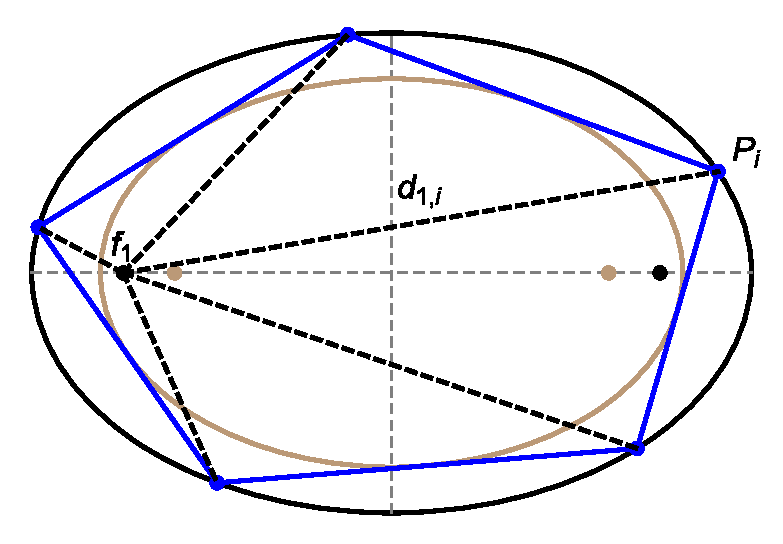
\includegraphics[width=.6\textwidth]{pics/0060_spoke_sum.eps}
    \caption{Over the homothetic family, the sum of distances $d_{1,i}=|P_i-f_1|$ is invariant, where $f_1$ is a focus of the outer ellipse.}
    \label{fig:spoke-sum}
\end{figure}

%\section{Summary}

\begin{table}
\begin{tabular}{|l|l|l|l|l|l|}
\hline
id & system & outer conic & inner conic & \makecell[lt]{$N=3$\\invariants} & \makecell[lt]{$N>3$\\holds?} \\
\hline
0 & billiard & ellipse $(a,b)$ & confocal caustic & $L,J,r/R,\color{red}\sum\cos$ & $L,J,\color{red}\sum\cos$ \\
1 & inner circle & ellipse $(a,b)$ & circle $r=\frac{{a}{b}}{a+b}$ & $R,r/R,\color{red}\sum\cos$ & $\color{red}\sum\cos$ \\
2 & outer circle & $R=(a+b)$ & ellipse $(a,b)$ & $\sum{s_i^2},\color{red}\prod\cos$ & $\sum{s_i^2},\color{red}\prod\cos$ \\
\textbf{3} & \textbf{homothetic} & \textbf{ellipse $(a,b)$} & \textbf{ellipse $(a/k,b/k)$} & $A,\sum{s_i^2},\omega,\color{red}\sum\cot$ & $A,\sum{s_i^2},\color{red}\sum\cot$ \\
4 & $X_4$ stationary & ellipse $(a,b)$ & ellipse $(a_0,b_0)$ & $X_4=0$ & pseudo-$X_4$ = 0 \\
\hline
\end{tabular}
\end{table}

%\begin{figure}
%    \centering
%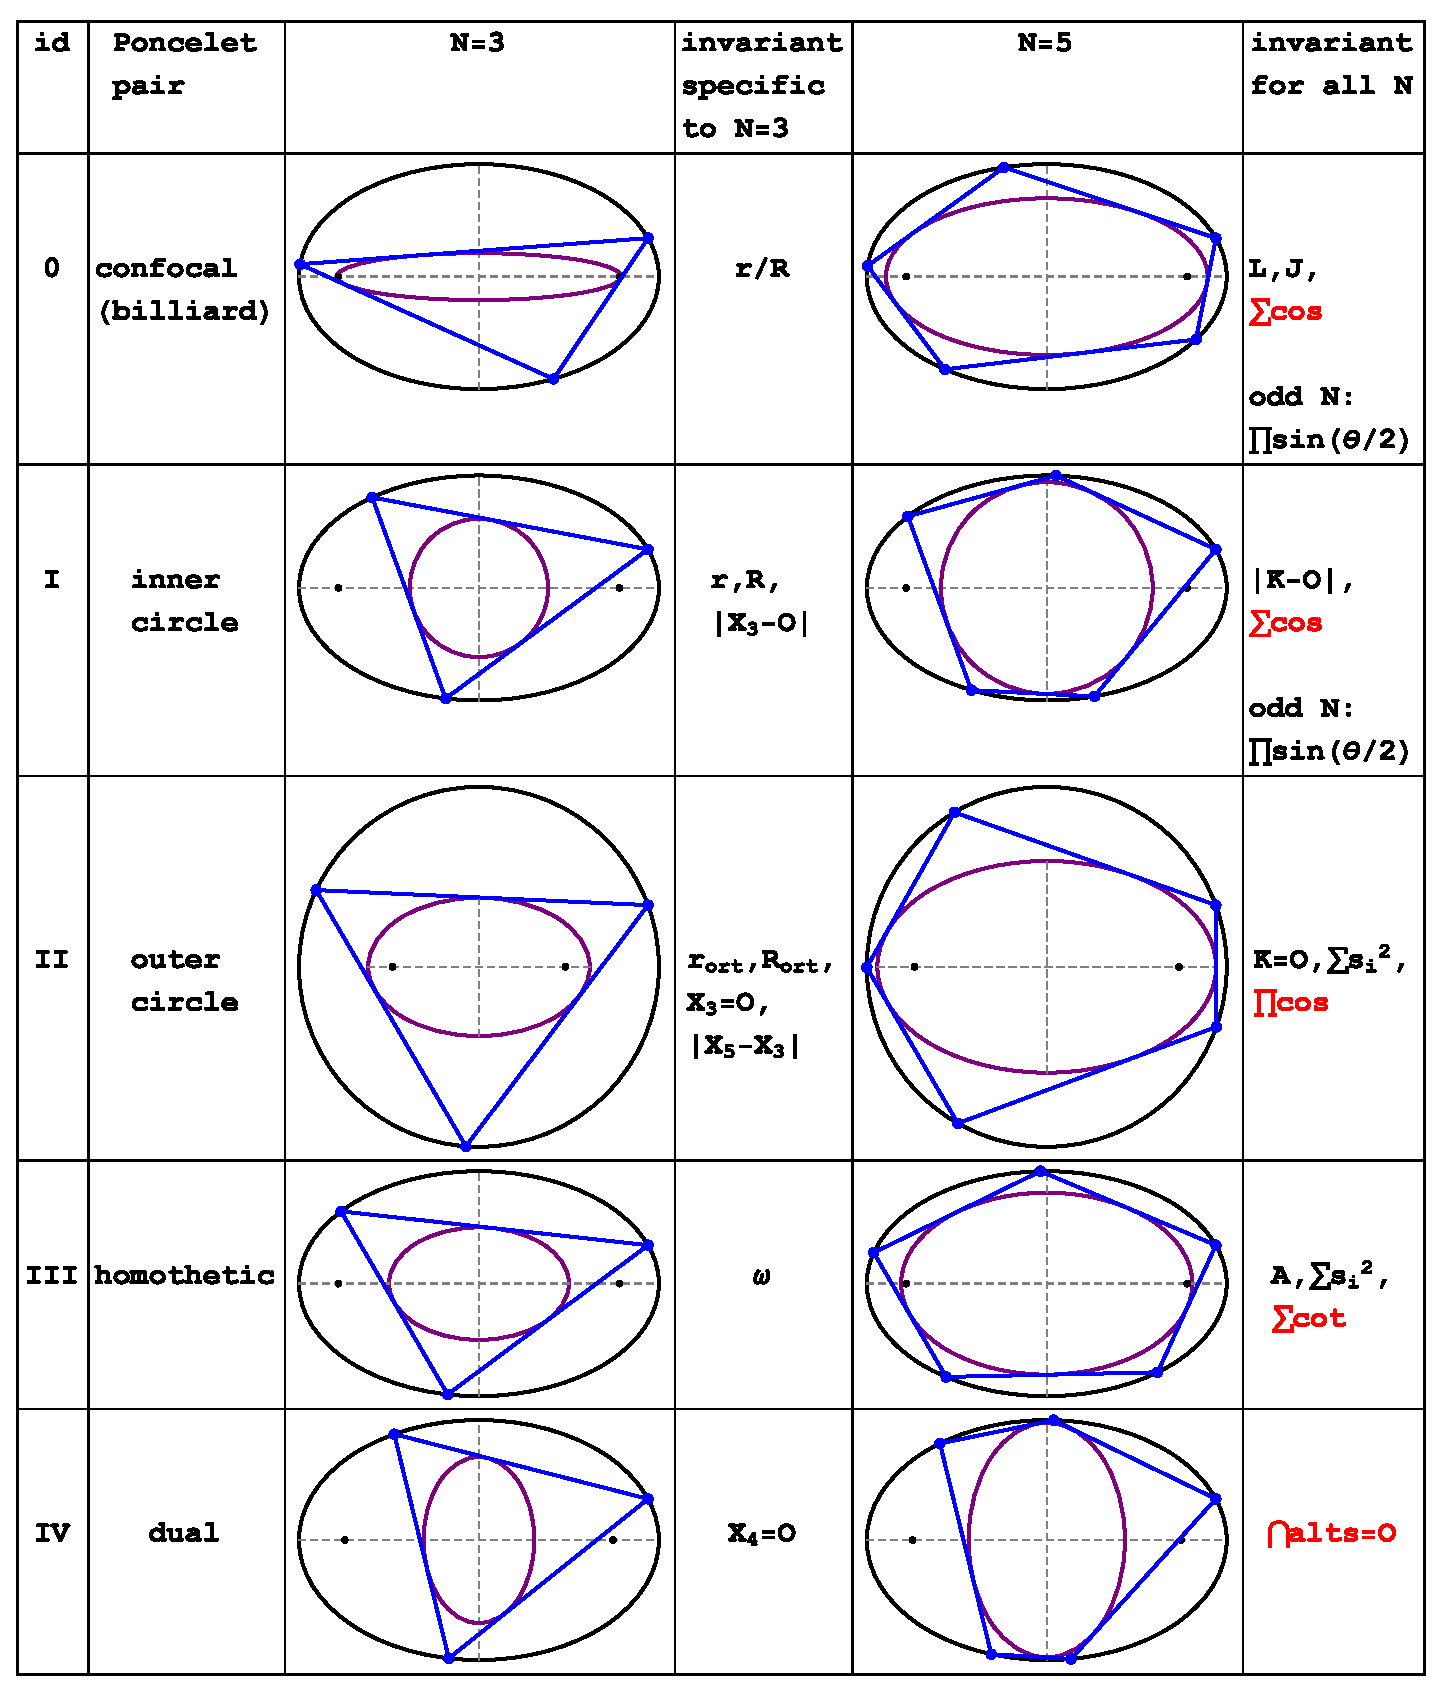
\includegraphics[width=\textwidth]{pics/0060_all_systems.eps}
%    \caption{}
%    \label{fig:all-systems}
%\end{figure}

\section{Video Table}
\label{sec:video-table}
Animations illustrating some phenomena herein are listed on Table~\ref{tab:playlist}.

\begin{table}[H]
\small
\begin{tabular}{|c|l|l|}
\hline
id & Title & \textbf{youtu.be/<.>}\\
\hline
01 & {Invariants of Poncelet N-Periodics in the Homothetic Pair} &
\href{https://youtu.be/2PdsC3CcqaE}{\texttt{2PdsC3CcqaE}}\\
02 & {Invariant Brocard Angles over 3-Periodics in the Homothetic Pair} & \href{https://youtu.be/2fvGd8wioZY}{\texttt{2fvGd8wioZY}} \\
03 & {Locus of Brocard Points over Homothetic 3-Periodics} & \href{https://youtu.be/13i3JGY-fK4}{\texttt{13i3JGY-fK4}}\\
\hline
\end{tabular}
\caption{Illustrative videos. The last column is clickable and provides the YouTube code.}
\label{tab:playlist}
\end{table}

\section*{Acknowledgements}
\noindent We would like to thank S. Tabachnikov and A. Akopyan for valuable insights. The second author is fellow of CNPq and coordinator of Project PRONEX/ CNPq/ FAPEG 2017 10 26 7000 508.

\appendix

%\section{Homothetic N-Periodic Vertices}
%Let $P_1(t)=(x_1,y_1)=(a\cos{t},b\sin{t})$. Then $P_{k+1}=(x_{k+1},y_{k+1})$, $k=0...(N-1)$ are given by:

\textcolor{red}{ronaldo}
\[ P_{k+1}=\left[a\cos \left( {\frac {2\,\pi\,k+tN}{N}} \right) ,b\sin \left( {\frac {
2\,\pi\,k+tN}{N}} \right) \right]
\]

%\label{app:explicit}

%\section{Classic Invariants for Any Concentric Poncelet}
%Consider a pair of ellipses
\[\frac{x^2}{a^2}+\frac{y^2}{b^2}-1=0,\;\;\frac{x^2}{a''^2}+\frac{y^2}{b''^2}-1=0. \]
The right Poncelet map is defined by
\begin{align*}
    P_r(x_1,y_1)& = (P_x,P_y)\\
    P_x&= {\frac {- \left( {a}^{2}{b}^{2}+{a}^{2}b''^{2}-a''^{2}{b
}^{2} \right)  \left( {a}^{2}{b}^{2}-{a}^{2}b''^{2}-a''^
{2}{b}^{2} \right) x_1+2\,{a}^{2} \left( {a}^{2}{b}^{2}-{a}^{2}{b''
}^{2}+a''^{2}{b}^{2} \right)  \,y_1 W }{4\,{b}^{2} \left( ab''-a''\,b \right)  \left( ab''+a''\,b \right) x_1^{2}+
 \left( {a}^{2}{b}^{2}-{a}^{2}b''^{2}+a''^{2}{b}^{2}
 \right) ^{2}}}\\
 P_y&={\frac {-2\,{b}^{2} \left( {a}^{2}{b}^{2}+{a}^{2}b''^{2}-a''^{2}{b}^{2} \right)  x_1W \varepsilon- \left( {a}^{2}{b}^{2}-{a}^{2}b''^{2
}+a''^{2}{b}^{2} \right)  \left( {a}^{2}{b}^{2}-{a}^{2}b''^{2}-a''^{2}{b}^{2} \right) y_1}{4\,{b}^{2} \left( ab''-a''\,b \right)  \left( ab''+a''\,b \right) x_1^{2}+
 \left( {a}^{2}{b}^{2}-{a}^{2}b''^{2}+a''^{2}{b}^{2}
 \right) ^{2}}}\\
 W&=\sqrt {a''^{2}{y_1}^{2}+b''^{2}x_1^{2} -a''^{2}b''^{2}},\;\;\;\varepsilon=\mathrm{sign}(y_1)
\end{align*} 

The left   Poncelet map is given by
\begin{align*}
    P_l(x_1,y_1)& = (Q_x,Q_y)\\
    Q_x&= {\frac {- \left( {a}^{2}{b}^{2}+{a}^{2}b''^{2}-a''^{2}{b
}^{2} \right)  \left( {a}^{2}{b}^{2}-{a}^{2}b''^{2}-a''^
{2}{b}^{2} \right) x_1-2\,{a}^{2} \left( {a}^{2}{b}^{2}-{a}^{2}{b''
}^{2}+a''^{2}{b}^{2} \right)  \,y_1 W}{4\,{b}^{2} \left( ab''-a''\,b \right)  \left( ab''+a''\,b \right) x_1^{2}+
 \left( {a}^{2}{b}^{2}-{a}^{2}b''^{2}+a''^{2}{b}^{2}
 \right) ^{2}}}\\
 Q_y&={\frac {2\,{b}^{2} \left( {a}^{2}{b}^{2}+{a}^{2}b''^{2}-a''^{2}{b}^{2} \right)  x_1W\varepsilon- \left( {a}^{2}{b}^{2}-{a}^{2}b''^{2
}+a''^{2}{b}^{2} \right)  \left( {a}^{2}{b}^{2}-{a}^{2}b''^{2}-a''^{2}{b}^{2} \right) y_1}{4\,{b}^{2} \left( ab''-a''\,b \right)  \left( ab''+a''\,b \right) x_1^{2}+
 \left( {a}^{2}{b}^{2}-{a}^{2}b''^{2}+a''^{2}{b}^{2}
 \right) ^{2}}}\\
 W&=\sqrt {a''^{2}{y_1}^{2}+b''^{2}x_1^{2} -a''^{2}b''^{2}},\;\;\;\varepsilon=\mathrm{sign}(y_1)
\end{align*}

The measure defined by
\[ d\eta=-{\frac {{b}^{2}{  dx}}{y\sqrt { \left( -b''^{2}+{y}^{2}
 \right) a''^{2}+b''^{2}{x}^{2}}}}={\frac {{a}^{2}{  dy}}{x \sqrt { \left( -b''^{2}+{y}^{2}
 \right) a''^{2}+b''^{2}{x}^{2}} }}\]
 is invariant by the Poncelet map.


%\label{app:concentric-poncelet}

\section{Table of Symbols}
\begin{table}[H]
\small
\begin{tabular}{|c|l|l|}
\hline
symbol & meaning & note \\
\hline
$\E,\E_c$ & outer and inner homothetic ellipses & \\
$N$ & number of Poncelet vertices & \\
$O$ & center of concentric pair & \\
$a,b$ & semi-axes of $\E$ & \\
$a_c,b_c$ & semi-axes of $\E_c$ & $(a_c,b_c) = \cos(\pi/N) (a,b)$ \\
$P_i,\theta_i$ & Poncelet vertices and angles & $i=1,...,N$\\
$f_1,f_2$ & foci of the outer ellipse & \\
$d_{1,i},d_{2,i}$ & distance from $P_i$ to $f_1,f_2$ & \\
$s_i$ & ith sidelength & $|P_{i+1}-P_i|$, $i+1$ mod $N$\\
$A,L$ & area and perimeter & $\sum{s_i}$ \\
$L_{2}$ & sum of squared sidelengths & $\sum{s_i^2}$ \\
$\omega$ & Brocard angle ($N=3$) & $\cot\omega=L_{2}/(4A)=\sum\cot{\theta_i}$ \\
\hline
\end{tabular}
\caption{Symbols used.}
\label{tab:symbols}
\end{table}

\label{app:symbols}

\bibliographystyle{maa}
\bibliography{references,authors_rgk} 
 \vskip 1cm
% \address
{
\noindent Sergey Galkin, \texttt{cotangente@galkin.org.ru} \\
Departamento de Matemática\\
% Pontifícia Universidade Católica do Rio de Janeiro
PUC-Rio\\
%Rua Marquês de São Vicente 225, Gávea,
Rio de Janeiro, RJ, Brazil, 22451-900
 
\vskip .5cm
\noindent Ronaldo Garcia, \texttt{ragarcia@ufg.br} \\ 
 Instituto de Matemática e Estatística\\
Universidade Federal de Goiás\\
Goiânia, GO, Brazil, 74690-900

\vskip .5cm
\noindent Dan Reznik, \texttt{dreznik@gmail.com} \\ 
 Data Science Consulting\\
Rio de Janeiro, RJ, Brazil, 22210-080
}
 

\end{document}
